\documentclass{article}


% \title{Cognitive syntax}

\title[Composition, not infinity]{Composition, not infinity: The irrelevance of recursion to theories of language}

\author{Edward Gibson\affiliation{Department of Brain and Cognitive Sciences, MIT}}

\graphicspath{ {./figures/} }

\begin{document}

\maketitle

\begin{abstract}

\cite{hauser2002faculty} famously proposed recursion to be core to human language. The present paper explains why Hauser et al.'s written proposal rightly equates recursion with syntactic self-embedding, following \cite{pullum2020theorizing}, and the sense in which self-embedding is the mechanism that generates the discrete infinity attested in many languages. This point is important because I then report recent email exchanges with Chomsky in which he clarifies that he thinks Dan Everett intentionally mis-characterized not the linguistic data of Pirahã, but what was intended in \cite{hauser2002faculty}. I argue that Chomsky’s accusation here is incorrect. That is, I think it’s clear what is meant by what was written in Hauser et al.'s (2002) paper and Everett and many others discussed those ideas appropriately, following the text written in the paper.  Then I move to a discussion of Pirahã itself: Dan Everett proposed that perhaps this language does not have the property of syntactic self-embedding, and therefore provides a counterexample to Hauser et al.'s (2002) universality claims. I will summarize the evidence that I know which seeks to evaluate this question and conclude that there is no strong evidence for recursion in Pirahã syntax. However, I emphasize that this is a difficult question to decide, although the independent claims of other languages without self-embedding make it much more plausibly true of Pirahã. In the final section, I provide an alternative to syntactic self-embedding as being a core component of human grammar: the existence of compositionality in language systems allows compression of what we need to communicate. A small lexicon and grammar gives rise to astronomically large numbers of potential utterances, and whether this set is infinite or not is irrelevant to anything about human nature. I conclude that recursion has been an irrelevant side-track in the theory of language.

\end{abstract}

\section{Introduction: The recursion claim from Hauser, Chomsky \& Fitch (2000)}

\itdopt{fix all citations, use citet = author citew = work citep = in brackets, Page numbers:
  (Gibson, 2003: 123) apply to whole volume, redo all tables in the volume according to LangSci
  style, Abbreviations all go to the end in a certain style as table}

\cite{hauser2002faculty} argued that the grammars for human languages are recursive, such that (more important components for my purposes are in bold):

\begin{quote}
\emph{All approaches agree that a core property of FLN (Faculty of Language, Narrow) is recursion, attributed to narrow syntax in the conception just outlined. FLN takes a finite set of elements and yields a potentially infinite array of discrete expressions. This capacity of FLN yields discrete infinity (a property that also characterizes the natural numbers).} Each of these discrete expressions is then passed to the sensory-motor and conceptual-intentional systems, which process and elaborate this information in the use of language. Each expression is, in this sense, a pairing of sound and meaning. It has been recognized for thousands of years that language is, fundamentally, a system of sound-meaning connections; the potential infiniteness of this system has been explicitly recognized by Galileo, Descartes, and the 17th-century ``philosophical grammarians'' and their successors, notably von Humboldt. One goal of the study of FLN and, more broadly, FLB is to discover just how the faculty of language satisfies these basic and essential conditions.

\emph{The core property of discrete infinity is intuitively familiar to every language user. Sentences are built up of discrete units:  There are 6-word sentences and 7-word sentences, but no 6.5-word sentences.  There is no longest sentence (any candidate sentence can be trumped by, for example, embedding it in `Mary thinks that  \ldots '), and there is no nonarbitrary upper bound to sentence length.  In these respects, language is directly analogous to the natural numbers (see below). } \citep[1571]{hauser2002faculty}
\end{quote}

In fact, as was widely discussed afterwards, there was no definition of ``recursion'' in \cite{hauser2002faculty};  They simply give an example, and ask the reader to infer what they probably mean.  
Here I follow \cite{pullum2020theorizing}  in assuming that a reasonable interpretation of what  \cite{hauser2002faculty} meant by recursion in a language is \textit{having syntactic devices that could in principle permit the construction of sentences of arbitrary length}.  I will refer to  this idea as \emph{syntactic self-embedding}.  The motivation for this interpretation is given in the following section.

\subsection{Elaborating Hauser, Chomsky \& Fitch's (2002) proposal in context-free grammar terms}

Because Chomsky and colleagues worked on phrase structure approaches to natural language syntax, here I elaborate how syntactic self-embedding in the grammar of such a formalism is equivalent to allowing the generation of utterances of unbounded length. A context-free phrase-structure grammar consists of a tuple (T, N, S, R), such that:

\begin{itemize}
    \item T is a finite set of terminal symbols: the words, that make up the lexicon or dictionary
    \item N is a finite set of non-terminal symbols
    \item S $\epsilon$ N is the start symbol
    \item R is a finite set of rules of the form X → $\alpha$, where X $\epsilon$ N, and $\alpha$ is a sequence of symbols drawn from T or N
\end{itemize}

A context-free phrase-structure grammar derivation is the recursive expansion of non-terminal symbols in a string by rules in R, starting with S. A derivation tree is the history of those rule applications (see \cite{chomsky1959certain, lewis1998elements, hopcroft2001introduction}).

A simple corpus of a few English sentences is given in \exref{corpus1}. A lexicon (a set of terminal symbols) T for this corpus is given in \exref{lexicon1}. And a rule set R that can generate the corpus in \exref{corpus1} is provided in \exref{cfg1}:

\eal
\label{corpus1}
\ex\label{corpus1a} The girl saw the dog.
\ex\label{corpus1c} Mary thinks that the girl saw the dog.
\ex\label{corpus1d} Alison says that Mary thinks that the girl saw the dog.
\zl

\ea
\label{lexicon1}
A Lexicon T:
\begin{verbatim}
Name → Mary, Alison
N → girl, dog
Det → the, a
V_NP → saw, liked
V_S → thinks, believes, says
\end{verbatim}
\z

\ea
\label{cfg1}
A rule set R:
\begin{verbatim}
1. S → NP VP
2. NP → Name
3. NP → Det N
4. VP → V_NP NP
5. VP → V_S that S
\end{verbatim}
\z

In phrase-structure terms, a category B is said to be \textit{embedded} within another category A if B combines with some other category to make A: this is simple compositionality within phrase structure.  The determiner (Det) \textit{the} can combine with the noun (N) \textit{girl} (according to rule 3) in order to form an NP that generates the string \textit{the girl}. The categories Det and N are then \textit{embedded} within the category NP.

A similar expansion applies to generate the NP \textit{the dog}. In order to form the VP that generates the string \textit{saw the dog}, we combine the V$_{NP}$ \textit{saw} with the NP \textit{the dog} according to rule 5. And finally, the NP \textit{the girl} combines with the VP \textit{saw the dog} to form an S category, according to rule 1, now covering the entire string \textit{the girl saw the dog} in \exref{corpus1a}.  This set of expansions is represented in the tree structure below:

\begin{center}
\Tree [.S [.NP [.Det the ] [.N girl ] ] [.VP [.V\sub{NP} saw ] [.NP [.Det the ] [.N dog ] ] ] ]

\end{center}

If the rules of the grammar are such that the category A can dominate another node of category A, then we have \textit{self-embedding} of A within A. The grammar in \exref{cfg1} has three instances of self-embedding: The category S expands to another S, through rules 1 and 6: an S expands to an NP and a VP in rule 1; and a VP expands to a V$_{S}$ and then a further S category in rule 5. We can generate arbitrarily long sentences using these rules, as \cite{hauser2002faculty} indirectly suggest. Parses for self-embedded examples like \exref{corpus1c} and \exref{corpus1d} according to the above grammar are provided below:

\begin{center}
\Tree [.S [.NP [.Name Mary ] ] [.VP [.V\sub{S} thinks ] that 
[.S [.NP [.Det the ] [.N girl ] ] [.VP [.V\sub{NP} saw ] [.NP [.Det the ] [.N dog ] ] ] ] ] ]

\hspace*{40pt}

\Tree [.S [.NP [.Name Alison ] ] [.VP [.V\sub{S} says ] that [.S [.NP [.Name Mary ] ] [.VP [.V\sub{S} thinks ] that 
[.S [.NP [.Det the ] [.N girl ] ] [.VP [.V\sub{NP} saw ] [.NP [.Det the ] [.N dog ] ] ] ] ] ] ] ]

\end{center}

Within context-free phrase-structure, it is only possible to generate utterances of unbounded length through syntactic self-embedding in the grammar.  To see this, first consider a grammar where we have syntactic self-embedding (as in the example above). There is clearly no limit to the number of times that the syntactic self-embedding can apply.  In our example, we can apply the category VP to generate an S, which generates a VP as many times as we like.  As long as one of VP or S (or both) is associated with the generation of at least one independent nonterminal, then we can generate a sentence of arbitrary length. Let's consider standard human language phrase structure, like X-bar theory \citep{jackendoff1977x}, such that each nonterminal is associated with at least one distinct terminal. That is, a VP in our grammar is always associated with a kind of verb (a $V_{S}$ or $V_{NP}$), which expands to exactly one terminal. Thus, there is no bound to the length of an utterance in a grammar with syntactic self-embedding.

Now let's consider the case of a grammar with no syntactic self-embedding, with $M$ nonterminal symbols. In such a grammar, the strings generated by the grammar \textit{must} be finite, because if you follow any path of nonterminals to their expansion as terminals you can never get to the same nonterminal twice (by hypothesis). Because there are $M$ nonterminals, this means that every path down the tree must be finite. Assuming that each terminal category expands to at most $k$ terminals (usually only one terminal per terminal category), this means that the length of the longest utterance is bounded by $M*k$. This also means that the set of sentences is finite.

Hence allowing sentences of unbounded length within a context-free phrase structure grammar is
equivalent to having syntactic self-embedding in the context\hyp free representation of natural language.  This is why we follow this interpretation of \cite{hauser2002faculty}.


\subsection{Everett's claim with respect to Pirahã grammar}

\cite{everett2005cultural} proposed that Pirahã does not have syntactic devices that could in principle permit the construction of sentences of arbitrary length. In particular, Everett claimed that the Pirahã language is \textit{finite}, with sentences of relatively small, finite length \citep{everett2012does}. This means that Pirahã would have no rules like the left- or right-branching rule sets, or center-embedded rule sets.  This does not mean that the set of sentences is small, however.  Even if each sentence is short in length, there can be an astronomically large number of them, as discussed below in Section~\ref{irrel_recursion_sec}.\footnote{\cite{everett2005cultural} also argued that features of Pirahã grammar follow from its culture.  While some version of this general hypothesis might be on the right track (see e.g., \cite{gil2021tense}, the particular cultural-grammar hypothesis that Everett makes here -- the immediacy of experience hypothesis -- seems implausible.  In any case, I will not discuss the orthogonal question of grammar-culture connections here.  Rather, I stick closely to generative capacity of Pirahã, and whether this language might have a syntactic  self-embedding device, but not why or why not.}

Note that even with no self-embedding in the syntax, we can express recursive meanings, as in \exref{rec_meaning}:

\eal
\label{rec_meaning}
\ex \label{rec_meaning1} Alison says that Mary thinks that the girl saw the dog.
\ex \label{rec_meaning2} Alison says the following. Mary thinks the following. The girl saw the dog.
\zl

\noindent
So the English doubly right-branching embedded sentence \exref{rec_meaning1} can be rephrased as the three separate utterances in \exref{rec_meaning2}. 
 Hence \cite{hauser2002faculty}’s claim is about the \textit{syntax} of utterances, and \cite{everett2005cultural}’s claim is about Pirahã syntax, not meaning.

\subsection{Some terminological confusion from Nevins et al. (2009)}

Over the years there has been some terminological confusion over what \cite{hauser2002faculty} meant by ``recursion'', either (a) self-embedding of a syntactic category, thus allowing for sentences of unbounded length, and a language with an unbounded number of sentences \citep{everett2005cultural}; or (b) ``merge'': effectively compositionality of any two syntactic elements \citep{nevins2009evidence}: \textit{``In a model with category-neutral Merge, however, a language that lacks recursion would be considerably more exotic. No sentence in such a language could contain more than two words. Pirahã is manifestly not such a language.''} \citep[366]{nevins2009evidence}.

If the ``merge'' definition results in a grammar with syntactic devices which permit unbounded sentence lengths, then this definition reduces to (a), syntactic self-embedding. On the other hand, if the ``merge'' definition does not allow syntactic devices which permit unbounded sentence lengths, there is no debate (as \cite{nevins2009evidence} observe): all human languages have compositionality (hence ``merge'' in their syntactic terms). In any case, \cite{everett2005cultural} is assuming definition (a): syntactic self-embedding definition, because that’s what the \cite{hauser2002faculty} quoted above says. What \cite{hauser2002faculty} care about is a grammar with devices that allow sentences of unbounded length.

\subsection{Chomsky claims that Everett intentionally misinterpreted what was intended in \cite{hauser2002faculty}}

An alternative kind of response to Everett’s claim about Pirahã is to claim that self-embedding may be \textit{available} in all languages, but not all languages use it. This is \cite{jackendoff2014what}’s view: they propose that there may be languages whose grammars do not result in self-embedded structures.

In fact, as of 2019, this is Chomsky’s claim about what was intended in \cite{hauser2002faculty}, according to an email exchange that I had with him then. The way that this email exchange started was that I wrote to Chomsky asking if he had called Dan Everett ``fraudulent'', because Dan had been told by students that Chomsky had told them this. Chomsky had written the following in an email to a student (which was shared with me, and which I sent to Chomsky, and which he acknowledged as being his):

\begin{quote}
    \textit{The Pirahã story is mostly fraud \ldots  By fraudulently claiming to have refuted assumptions about recursion in language, Everett managed an impressive PR triumph, but nothing beyond that.}  Email from Noam Chomsky, September 2019.
\end{quote}

I asked Chomsky to clarify in what sense that Everett was behaving ``fraudulently''. In the email discussion that followed, it became clear that Chomsky thought that Everett intentionally misinterpreted the \cite{hauser2002faculty} paper.  That is, Chomsky believes that what is stated in the \cite{hauser2002faculty} paper is that it is irrelevant that there may be exceptions to the generalization that he and his authors were providing: he said that the intended claim was not that recursion is universally \textit{used}. Chomsky said that what was intended was that recursion is universally \textit{available} for human languages. According to Chomsky, Everett is behaving ``fraudulently'', because Chomsky believes that Everett knew what was intended in \cite{hauser2002faculty} and the literature that it cites, and Everett was intentionally saying something else, to serve his own purposes which Chomsky terms ``a PR triumph''. 

So yes, Chomsky did say Everett was behaving fraudulently, but in a non-standard use of the word, in my opinion. When I first heard that Chomsky thought that Everett was behaving fraudulently, I assumed that Chomsky thought that the claims about Pirahã were somehow made up, based on falsified data or analyses of some kind, because this is the typical sense of fraud in science.  But that was an odd idea with respect to the Pirahã, because the data are mostly non-quantitative, so it's hard to falsify anything in that domain in a technical way. Indeed, this was not Chomsky's sense of fraud here.\footnote{Chomsky's sense of fraud is particularly odd because it relies on Chomsky knowing what Everett intends, which is obviously impossible. That is, Chomsky would need to be certain that Everett believes that Chomsky meant that recursion is only universally \textit{available} for human languages, not necessarily present in all languages. In discussing this with Everett, it is clear that Everett does not believe this.}

Furthermore, while it may be the case that when writing \cite{hauser2002faculty}, Chomsky intended an interpretation whereby recursion is universally \textit{available} for human languages, that's not what Chomsky and his co-authors wrote.
% \footnote{\cite{pullum2023daniel} suggests that Marc Hauser may have written most of the article. This is a possible reason for the disconnect.  Perhaps Chomsky told Hauser what he intended, and Hauser wrote something different.  This of course does not excuse Chomsky's inappropriate accusations against Everett.} 
In particular, the original writing quoted above suggests that a universal property of language was intended. The line ``The core property of discrete infinity is intuitively familiar to every language user'' is explicitly about \textit{every language user} not \textit{every English user} or \textit{every Mandarin user}.  This is a claim about all speakers of any human language. Furthermore, the line ``There is no longest sentence  \ldots  and there is no nonarbitrary upper bound to sentence length.'' is not about any particular language. This is about human language in general. English is given only as an example. 

This was Everett’s interpretation of \cite{hauser2002faculty}, which I share. This is also every other researcher’s interpretation who I have ever talked to. I even have assigned the \cite{hauser2002faculty} paper to some classes to see what reading the students get, and they always get the same interpretation as Everett, in spite of never having read anything by Everett.  So I think it’s inappropriate to blame Everett for the ``universal'' interpretation of \cite{hauser2002faculty}: that interpretation comes from the text itself. 

A second response to Everett’s claim has been to suggest that Pirahã probably does have syntactic self-embedding, in the same way that English does. \cite{sauerland2018false} suggests that this is the case, based on experimental data that he gathered when visiting the Pirahã. I discuss in more detail in Section~\ref{sauerland_sec}.

\section{Does Pirahã have  syntactic devices that could in principle permit the construction of sentences of arbitrary length?}

The Pirahã are an indigenous people of the Amazon basin who are hunter\hyp gatherers, with little agriculture.  In early 2007, Mike Frank and I traveled with Dan Everett to work with the Pirahã to investigate aspects of Pirahã language and cognition. At that time, there were approximately 800 people in about six Pirahã villages. They had minimal contact or trade with outsiders. 

Mike Frank and I (in collaboration with Ev Fedorenko, who didn’t make the trip) ran several experiments trying to understand (a) Pirahã number terms and what they meant \citep{frank2008language}, and (b) elementary Pirahã syntax. But investigating a language’s syntax is complicated.  In collaboration with Eugenie Stapert (a graduate student working with Dan Everett at the time) and Jeanette Sakel (a postdoc working with Everett), we designed some simple methods to try to get participants to generate self-embedded structures, modeling our attempts on the syntax of English and related languages. In particular, we attempted to get Pirahã participants to generate potential self-embedded possessives and relative clauses, by asking them to describe - in their language - situations that we presented to them.

\subsection{Attempts at elicitation of possessive noun phrases}

In our attempt to elicit possessive noun phrases along the lines of ``Kóxoi’s father’s sibling’s child'', we showed a set of dolls to each of nine Pirahã participants, where the dolls were presented sequentially as in \exref{kohoi_ex}. The participants were told that each doll represented a Pirahã person (or animal, as there was also a dog). For example, the first doll in one set of dolls was an adult male named ``Kóxoi’' (a possible Pirahã name). Each time that a new doll was presented, We told the participant the relationship between the new doll and the previous one, and we asked them to describe the current doll in relation to the initial doll.  So, for example, if the first doll was called Kóxoi, the second doll would have a close relationship to Kóxoi, such as his spouse. We asked the participant to tell us who this was, and all participants  replied with an order of the name that was given (such as Kóxoi) and the relation, such as ``Kóxoi spouse'' or ``Kóxoi brother'' or ``brother Kóxoi''. Of 23 trials that we performed, 17 were ordered modifier-head (like ``Kóxoi spouse''), and 6 were ordered head-modifier (like ``spouse Kóxoi'').

Although these examples could in principle be syntactic self-embedding of a noun phrase within a noun phrase, they could also be the result of a rule that allows only two nouns to combine, and does not allow arbitrary embedding.  Hence examples of just two combined nouns does not provide strong evidence of syntactic self-embedding.

\eal
\label{kohoi_ex}
\ex \label{kohoi_ex1} This is Kóxoi. (pointing to doll 1, male)\\
Who is this?
\ex \label{kohoi_ex2} He has a spouse. (pointing to doll 2, female)\\
Who is this?
\ex \label{kohoi_ex3} She has a parent. (pointing to doll 3, male)\\
Who is this?
\ex \label{kohoi_ex4} He has a dog. (pointing to doll 4, a dog)\\
Who is this?
\zl

The presentation of the third doll was intended as a test of syntactic self-embedding in Pirahã possessive nominals.  We told the participant that this doll had another close relationship with doll 2, such as the parent of doll 2.  We then asked the participants to describe the third doll in relation to the first doll (e.g., Kóxoi).  Of the 34 responses at this level, 14 expressed only a single relationship between two of the dolls.  Of the remaining 20 responses, only 8 expressed relationships among the three dolls appropriately, but none of these were plausibly syntactic self-embedding in Pirahã.  Rather, they were statements like ‘This is Kóxoi, this (his) parents sibling’ or ‘Koxoi’s sibling, he has a spouse’.

The fourth doll also tested the potential existence of syntactic self-embedding in Pirahã possessive nominals. Our nine participants failed to produce any utterances that linked the fourth doll to the first through labels for the second and third, even with multiple clauses.  They also did not produce any sequences that could be plausibly analyzed as syntactically embedded connecting three together. The longest sequence that were connected in the same syntactic nominal was two nouns.

This particular study therefore failed to provide evidence that Pirahã speakers could combine sequences of more than two nouns compositionally, in possessive nominals.  This does not mean that Pirahã lacks such sequences; but it is suggestive in that direction.

\subsection{Attempted elicitation of relative clauses}

Our second attempt to elicit syntactic self-embedding in Pirahã consisted of an attempt to elicit relative clauses.  To do this, we used two of our dolls that we used to represent Pirahã people. We would show each doll to the participant, and tell them an event that each one took part in, as in \exref{piraha_rcs}:

\eal
\label{piraha_rcs}
\ex \label{piraha_rcs1} Doll 1: This person paddled a canoe.
\ex \label{piraha_rcs2} Doll 2: This person swam in the river.
\zl

We would then tell the participant that one of the dolls took part in a third event, as in:

\ea
\label{piraha_rcs3}
Doll 1: This person ate some farinha.
\z

We would then take the dolls away, and ask who took part in the last event: \textit{Who ate some farinha}?  If the Pirahã language includes relative clauses in its syntax, then it is possible that people might generate materials like \textit{The man who paddled the canoe ate some farinha}. But as discussed briefly above, a language does not need syntactic tools to represent such complex (embedded) meanings.  A language can represent such meanings using anaphoric elements (pronouns of various kinds) to link between separate simple syntactic elements, one for each clause.  This general strategy is sometimes called \textit{parataxis}.


\begin{table}
    \begin{tabular}{c c c c}
         Single Sentences & Parataxis & Did not follow instructions & Likely relative clause  \\
         \hline 
         35 & 13 & 22 & 0 
    \end{tabular}
    \caption{Number of instances of each type in attempted relative clause elicitation}
    \label{table1}
\end{table}

The 70 responses from our 9 participants on this task were distributed as in Table~\ref{table1}.  Of the 13 two-clause responses, all were likely parataxis, consisting of pairs of clauses like \textit{canoe paddle} and \textit{same eat farinha}, where the Pirahã word for \textit{same} connects the subjects of the two clauses.

For whatever reasons — bad designs, naiveté, complex or culturally odd meanings — we were unable to get participants to generate anything that might reasonably be analyzed as having self-embedded syntax. We therefore failed to provide evidence that there is self-embedded syntax in Pirahã.  But of course we did not provide strong evidence for the lack of self-embedded syntax either.

It is also worth noting that \cite{sakel2010piraha} investigated the use of the suffix ``-sai'' -- which had been proposed earlier by \cite{everett1986piraha} to be a sentence embedding marker -- and they found no evidence of syntactic self-embedding, in either spontaneous elicitation or in a sentence repetition task. Instead, \cite{sakel2010piraha} suggest that ``-sai'' is a discourse marker, which is not connected syntactically to the clause that it appears adjacent to.

\subsection{\citew*{futrell2016corpus}}

\citet{futrell2016corpus} analyzed a corpus of spoken Pirahã that Dan Everett and the previous missionary to the Pirahã -- Steve Sheldon -- had gathered, to see what the simplest syntactic re-write grammar might be, and whether that grammar had self-embedding. \cite{futrell2016corpus} parsed 17 Pirahã stories (13 by Sheldon in the 1970s, 4 by Everett in 1980—2009; 1149 sentences; 6830 words), and looked at the resulting structures for evidence of syntactic self-embedding. The full parsed corpus is available at http://osf.io/kt2e8 .

In this project, \cite{futrell2016corpus} looked for examples of syntactic self\hyp embedding in a range of kinds of examples that are typically analyzed as syntactic self-embedding in English, including the following:

\begin{itemize}
    \item Relative clauses: No examples.
    \item Coordination: Conjunctions / disjunctions: No examples 
    \item Possessive structures: No examples
    \item Nominalizers and complementizers: No examples
    \item Reported speech: Possible examples; but the examples could also be analyzed as a sequence of non-embedded utterances
\end{itemize} 

As indicated above, we found no evidence for syntactic self-embedding in the form of relative clauses, coordination structures, possessive structures, nominalizers or complementizers (subordinate clause markers). The one case that might plausibly be analyzed as syntactic self-embedding was \textit{reported speech}, such that the reported content of the speech (what was said) frequently appears immediately following a form of the verb \textit{gá} (``speak'' / ``say''). In 183 of the 191 instances of this verb in the corpus, the content of the reported speech immediately followed. In the remaining 8 instances, the verb was used clearly intransitively, with no following reported speech. It is possible to analyze this verb as always being intransitive, with the content of the reported speech indicated but not necessarily an argument of the verb, as in:  \textit{Mary spoke.  Bill will be coming.}  The listener can infer that the following clause is what Mary said.  

Of course, it is also possible to analyze the reported speech as an argument of the verb \textit{gá} (``speak''), in which case Pirahã would have at least this case of syntactic self-embedding.  But since this seems to be the only case where syntactic self-embedding might be motivated, it is also possible to analyze this case without syntactic self-embedding.

So overall, the corpus evidence do not provide strong evidence for syntactic self-embedding. Of course there are limitations to this work, such as the fact that this is a small corpus.  Perhaps obvious instances of syntactic self-embedding are not present in such small corpora.  Another limitation of this work is that there is no control corpus from another language whose participants are matched on socio-economic status.  That is, it is possible that aspects of education drive the desire / need to talk in a syntactically embedded way.  Perhaps we would find few instances of syntactic embedding in a corpus of speech among people who lack general education about other cultures.

\subsection{\citew{sauerland2018false}}
\label{sauerland_sec}

In contrast to \cite{futrell2016corpus}, \cite{sauerland2018false} purported to have found evidence of syntactic self-embedding in Pirahã, by gathering interpretations of experimental materials. In order to do this, Sauerland went to work with the Pirahã, and had two native speakers record materials of the following form, that he would then play to other Pirahã native speakers:\footnote{As noted by \cite{everett2019recursion}, there are issues with the Pirahã materials: it is not typical Pirahã language, probably because the translator that Sauerland used didn't speak good Pirahã. \cite{everett2019recursion} provide better Pirahã translations of the target materials. In any case, this problem is less of an issue than other problems with Sauerland's design and interpretation, to be discussed here.}

\eal
\label{sauerland_ex}
\ex \label{sauerland_ex1} Spoken by speaker 1 (Toe):\\
\begin{tabular}{l l l l}
ce & kahápe & ogéhiai & igeuo \\ 
I & have.been & stars & there\\
\end{tabular}

``I have been to the stars''

\ex \label{sauerland_ex2} Spoken by speaker 2:\\
\begin{tabular}{l l l l l l l l}
Toi & he & gái-sai & ce & kahápe & ogéhiai & igeuo \\
Toe & 3sg & say & 1sg & have.been & stars & there\\
\end{tabular}


i. subordinate interpretation: ``Toe said ‘I have been to the stars’.''\\
ii. co-ordinate interpretation: ``Toe talked, and I have been to the stars.''
\zl

Thus Speaker 1 (named ``Toe'') said \textit{I have been to the stars}, which is intended to be statement that is obviously impossible. The dependent measure was how the listeners interpreted Speaker 2's statement, which depended on how they would interpret the pronoun ``I'' (ce) in speaker 2’s statement. The pronoun ``I'' in speaker 2’s statement might refer to ``Toe'', giving  a subordinate interpretation. In English, this might correspond to sentences like \textit{Toe said ``I have been to the stars''}, or \textit{Toe said that he has been to the stars}. Or the listener might interpret``I'' as Speaker 2, to get a coordinate interpretation, corresponding to English materials like \textit{Toe said something and I have been to the stars.}  Critically for Sauerland, the coordinate interpretation is false in this scenario (Speaker 2 hasn’t been to the stars), while the subordinate interpretation is true (Toe did say that he had been to the stars).

Sauerland hypothesized that in order to get the subordinate interpretation, a language needs syntactic recursion. (This assumption is not actually correct; I return to this problem below.) Thus if people get the subordinate interpretation, then Pirahã must have syntactic recursion. Sauerland investigated this by asking participants if these sentences were true in the context. 

\cite{sauerland2018false} provided many of the details of his raw data, so we can visualize his results in \figref{fig:gibson:fig1}, where each shaded square represents the answers given by a Pirahã participant in his critical experiment and a control experiment. In this figure, the Y-axis indicates the number of embedded interpretations out of nine that a particular participant obtained, and the X-axis indicates the number of correct interpretations of the nine control materials (to be described below) that the participant got. There are 16 shaded squares: one for each participant, including two who happened to give the same pattern of subordinate and control responses.

\begin{figure}
%     \centerline{\includesvg[width=.7\textwidth]{gibson_figure1.svg}}
    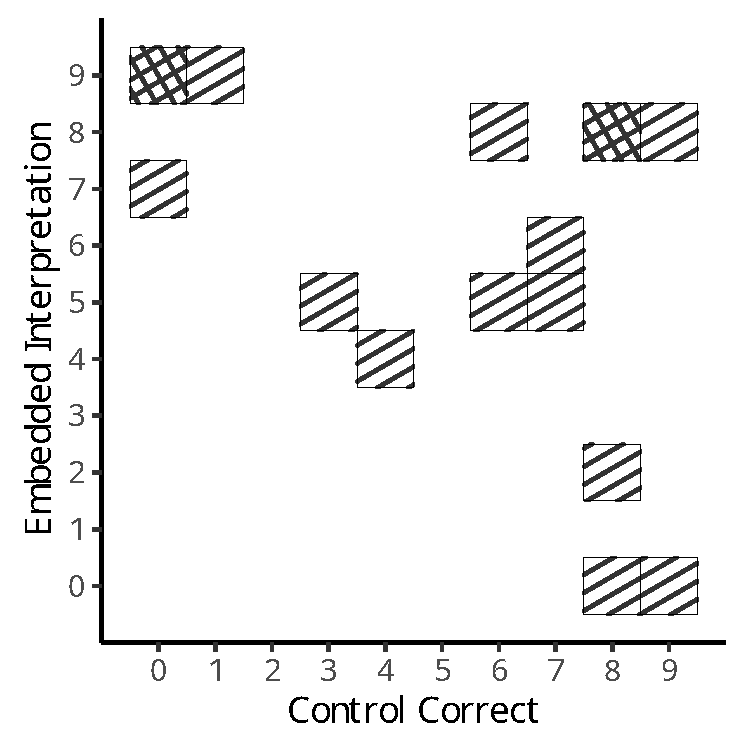
\includegraphics[width=.9\textwidth]{gibson_figure1.pdf}
    \caption{Each shaded square represents the answers given by a Pirahã participant in two sub-experiments conducted by \cite{sauerland2018false}. On the Y-axis are the number of embedded interpretations out of nine. On the X-axis are the number of correct interpretations of the control materials, also out of nine. There are 16 shaded squares one for each participant, including two who happened to give the same pattern of subordinate and control responses.  \newline \newline For Sauerland's data to be supportive of his hypothesis, participants would need to be in the upper right corner of the graph:  most passing the control test, and most showing evidence of an embedded interpretation.  Most participants are not in the upper right corner. Even if the data had been in the upper right corner, this would not be evidence of syntactic embedding, as discussed in the text. \newline \newline
    Data reported as presented in \cite{sauerland2018false}, replotted using \cite{r2023, wickham2016, ggpattern2022}. (Thanks to Moshe Poliak for this picture.)}
    \label{fig:gibson:fig1}
\end{figure}

We can see in the figure that there are more participants higher up on the Y-axis, indicating more responses favoring the subordinate interpretation. Sauerland ran a statistical test that suggested that this proportion was greater than chance, and he concluded that Pirahã has recursive syntax.

\subsubsection{Flaws in Sauerland's design and interpretation}

There are two major flaws with Sauerland’s reasoning here. First, we need to ensure that the participants understood the task. And second, contrary to Sauerland's assumption, a subordinate interpretation can come from either an embedded or a non-embedded syntax: there is no necessary connection between the two.  I address each of these two issues below in turn.

First, Sauerland doesn't speak Pirahã. So he needs some control to ensure that the participants understood the task. In order to address this potential issue, Sauerland included a set of nine control sentences, that had correct answers.  One such example is given in \exref{sauerland_ex_cont}:

\eal
\label{sauerland_ex_cont}
\ex \label{sauerland_ex1_cont} Spoken by speaker 1 (Toe):\\
\begin{tabular}{l l l l}
ce & kahápe & kahe’ai & igeuo \\ 
I & have.been & moon & there\\
\end{tabular}

``I have been to the moon''

\ex \label{sauerland_ex2_cont} Spoken by speaker 2:\\
\begin{tabular}{l l l l l l l l}
Toi & he & gái-sai & ce & kahápe & heesé & igeuo \\
Toe & 3sg & say & 1sg & have.been & sun & there\\
\end{tabular}

i. co-ordinate interpretation: ``Toe talked, and I have been to the sun.''\\
ii. subordinate interpretation: ``Toe said ‘I have been to the sun’.''
\zl

These materials are just like the target materials, except that Speaker 2 now refers to a different location that Speaker 1 (Toe) is purported to have visited.  So while Toe talks about the moon in his statement, Speaker 2 refers to the sun as the place that someone might have visited.  Now, Statement 2 is false, no matter whether the participant gets the subordinate or coordinate interpretation.  So participants need to have rejected all of these sentences uniformly.

The results from the control experiment are presented on the X-axis:  people who understood the task were the ones who got more control questions correct: the rightward people on the X-axis.  Note that there are many participants who get fewer than 6 or 7 of the control questions correct.  It's unclear what these participants thought was intended by the materials.  But whatever they thought, we should not be analyzing their data. Hence, Sauerland should only be analyzing participants’ data who understood the controls (e.g., at least 6 of 9 correct):  which is only 10 of the 16 participants: the ones on the right. When one analyzes these data, the participants are at chance at interpreting the experimental items in the subordinate reading.

So contrary to what Sauerland says, his Pirahã participants don’t actually reliably get the embedded interpretation. The ten participants who understood the task were completely at chance in that interpretation.

The second problematic issue in Sauerland's paper is that he assumes that answering ``true'' to the target materials necessitates a self-embedded syntactic structure.  This is not the case.  Alternatively, it could be that the meanings of the materials are biased towards a subordinate \textit{meaning}, whether or not there is self-embedded syntax.  We can test this hypothesis in English by giving people similar materials in English, but critically with no syntactic embedding.  \cite{everett2019recursion} did this with 20 participants on English translations of Sauerland's materials, as in \exref{ev_gib2019_ex}: 

\ea
\label{ev_gib2019_ex}
John: ‘I have been to the stars.’\\
Bill: John said something. I have been to the stars.
\z

The question is who does ``I'' refer to in Bill’s sentence:  John or Bill? Sauerland thinks that we can only get a referent to ``John'' through embedding in the syntax, such as ``John said that I have been to the stars.''  But In spite of the lack of syntactic embedding in the materials all participants answered ``true'' most of the time (98\% of trials), getting the embedded meaning interpretation, in spite of no embedded syntax.  Hence, people think ``I'' refers to John almost all the time in \exref{ev_gib2019_ex}, even with no embedded syntax

So, in spite of a non-embedded syntax, people get the embedded meaning, contrary to Sauerland’s assumption.  We don’t need recursive syntax to get the embedded meaning interpretation.  It appears that Sauerland's materials were biased towards an embedded meaning, independent of the syntax. Indeed, the Pirahã participants answered with a non-embedded interpretation far more often than English speakers did. It's hard to know why that might have been.  My guess is just that the materials and task are confusing for the participants.  They generally didn't know what they were supposed to do, and answered semi-randomly across people.

\subsection{Pirahã is not even exceptional in its syntactic structure}

Overall, my conclusions from \cite{futrell2016corpus} and \cite{sauerland2018false} are that we have no evidence for self-embedded syntax in Pirahã. This null result does not establish that there is no self-embedded syntax in Pirahã, but (a) several attempts to elicit it have not succeeded, (b) it is not obviously present in naturalistic corpora, and (c) it is not present according to the primary linguist who worked there.

It is worth observing that many other researchers have suggested that languages other than Pirahã might also lack self-embedding in the syntax. \cite{pullum2023daniel} documents several languages that had been provided as evidence of similar claims by researchers well before Everett, including Iatmul, Gunwinggu, Kathlamet, Mohawk, and some Pama-Nyungan languages. And more recently, \cite{gil2009much, jackendoff2014what, gil2023hierarchical} discuss Riau Indonesian, suggesting that this language may lack syntactic self-embedding; and \cite{jackendoff2014what} discuss how newly-formed sign languages may have similar properties \citep{goldin2005resilience, sandler2005emergence}.

Against this backdrop, HCF's claim is somewhat bizarre. How could they have proposed that ``recursion'' was known to ``all language users'' if so many languages have been argued not to have it? One possibility is that they were simply unaware of the typological data already reported in the field. But it is interesting to consider how their proposal would have been different if they had engaged this prior literature, and tried to find a universal that was empirically attested in all human languages. 

\section{The irrelevance of recursion / syntactic self-embedding to theories of grammar}
\label{irrel_recursion_sec}

Finally,  I return to the main point of this brief paper: Why did \cite{hauser2002faculty} focus on ``recursion'' (self-embedding in the syntax) anyway?  \cite{hauser2002faculty}’s claim is that being able to generate an \textit{unbounded} number of sentences is a critical feature of human languages, which gives rise to \textit{discrete infinity}, which they think is a crucial feature of human languages.  But why should generating an unbounded number of sentences be a feature of a human language?  This is not a feature that any language user can take advantage of. So clearly ``usefulness'' is not what Chomsky and colleagues have in mind as a design feature of human language (contrary e.g., a current claim in language: that language is evolved for efficient use e.g., \cite{gibson2019efficiency}).

Furthermore, the existence of potential exceptions to this claim (such as Pirahã) suggests that human languages need not generate an unbounded number of sentences in order to be useful as communication systems. Alternatively, maybe the useful feature of compositional (combinatorial) rules in human language is compression: the fact that having a grammar with generalizations over categories enables us to convey our ideas more efficiently. With categories of forms (words / morphemes), and rules to combine them, we can convey far more meanings than if we associate each complex meaning with an independent form. Compositionality can evolve in a linguistic system that is trying to be concise/learnable while having lots of meanings \citep{kirby2000syntax}.

% (Indeed,  \cite{nevins2009evidence} suggest that they think this is what \cite{hauser2002faculty} meant, even if it is not what \cite{hauser2002faculty} said.). 

Note that even with a finite language, we can convey an unfathomably large number of meanings. For example, suppose that there were $5000$ nouns in the lexicon, among other words. Suppose that there were 100 different syntactic sequences 20 words long, with 10 nouns in each sequence, such that each noun could go in any noun position as in \exref{ex1}. This gives at least 5,000$^{10}$ x 100 = 10$^{39}$ sequences, even ignoring the flexibility of all the other words in the sequences (represented as ``x$_i$'' for each). (See \cite{muller2016grammatical} for a similar point.)

\ea
\label{ex1}
100 sequences of 20 words, each with 10 nouns in a different set of positions across sequences; the sequences shown are arbitrary sequences from the set:\\
Sequence 1: N$_1$ x$_1$ N$_2$ x$_2$ N$_3$ x$_3$ N$_4$ x$_4$ N$_5$ x$_5$ N$_6$ x$_6$ N$_7$ x$_7$ N$_8$ x$_8$ N$_9$ x$_9$ N$_{10}$ x$_{10}$\\
Sequence 2: N$_1$ N$_2$ x$_1$ N$_3$ x$_2$ N$_4$ x$_3$ N$_5$ x$_4$ N$_6$ x$_5$ N$_7$ x$_6$ N$_8$ x$_7$ N$_9$ x$_8$ N$_{10}$ x$_9$ x$_{10}$\\
Sequence 3: N$_1$ x$_1$ N$_2$ N$_3$ x$_2$ N$_4$ x$_3$ N$_5$ x$_4$ N$_6$ x$_5$ N$_7$ x$_6$ N$_8$ x$_7$ N$_9$ x$_8$ N$_{10}$ x$_9$ x$_{10}$\\
. . .\\
Sequence 100: x$_1$ x$_2$ N$_1$ N$_2$ N$_3$ x$_3$ N$_4$ N$_5$ x$_4$ N$_6$ x$_5$ N$_7$ x$_6$ N$_8$ x$_7$ N$_9$ x$_8$ N$_{10}$ x$_9$ x$_{10}$
\z

There are 10$^{10}$ neurons in the brain and 10$^{50}$ atoms in the earth. These are inconceivably large numbers. There is no need to appeal to infinity / unboundedness to explain human language: large finite sets are sufficient to motivate a compositional grammar. Recursion or syntactic self-embedding is irrelevant to this argument.

Finally, the unboundedness of sentence length is an odd property for Chomsky and colleagues to propose as the most critical part of human grammar.  ``Arbitrarily'' long (or deeply nested) sentences are never actually realized, due to performance constraints. How could the critical property of human-like language be something like unboundedness, which isn’t ever seen? It's a bit like claiming that the defining feature of a car is that it can in principle go any speed, even though we only ever actually see it go two hundred miles per hour. This kind of theorizing is confused and simply can't be right. The critical aspects of human language will inevitably turn out to be features which are empirically observed in languages, not abstractions about infinity that no human mind actually realizes.

\printbibliography[heading=subbibliography,notkeyword=this]




\end{document}


